\documentclass[11pt,letterpaper]{article}
\usepackage[margin=0.90in]{geometry}
\usepackage{amsmath, amssymb}
\usepackage{times}
\usepackage{fancyhdr}
\pagestyle{fancy}
\usepackage{natbib}
\usepackage{titling}
\usepackage{setspace}
\usepackage{bm}
\usepackage{xcolor}
\usepackage{graphicx}
%\setlength{\textfloatsep}{-1pt}


\begin{document}
\begin{titlepage}
	\centering
	{\scshape\LARGE McMaster University \par}
	\vspace{1cm}
	{\scshape\Large Final year project for Datascience 780\par}
	\vspace{1.5cm}
	{\huge Predicting Diabetes in  Pima Indian Women \par}
	\vspace{2cm}
	{\Large\itshape by Nik Po\v cu\v ca\par}
	\vfill
	Instructor:  \par
	Dr. Sharon McNicholas 

	\vfill

% Bottom of the page
	{\large \today\par}
\end{titlepage}

\doublespacing

\section{Introduction}

Diabetes is an ongoing chronic illness that causes the body to have an inability to process glucose(sugar) by restricting or eliminating the kidney's ability to produce insulin. 
By 2025 the estimated prevalence of diabetes in Canada will increase to 5 million or $12.5$ of Canadians everywhere, not only putting Canadian lives at risk of premature death but cost alone is estimated to increase by $25 $ by 2025 \citep{diabetes}. Therefore the need to accurately predict diabetes is growing with data analysis at the forefront. The Pima Indians dataset contains a population of women who were at least 21 years old of Pima Indian heritage and living near Phoenix, Arizona. The population was tested for diabetes according to World Health Organization criteria and data were collected by the US National Institute of Diabetes\citep{pima}. This report contains a thorough set of analyses for the purposes of classifying diabetes based on covariates. First a look at each covariate and description of measurements is provided. Secondly, model methodology and description of model use is discussed. Furthermore, results from both training models and criteria for optimal model selection is provided. Finally, conclusions regarding the feasibility of the utilization of these models are discussed. 

\section{Pima Dataset}

The Pima dataset (Diabetes of Pima Indian Women) taken from the MASS package \citep{pima_d}
in the programming langauge R \citep{Rprog} contains $ 532$ complete records after dropping the (mainly missing) data on serum insulin.  The dataset contains $7$ covariates decribed in Table \ref{covDes}.

\begin{table}[!h]
\label{covDes}
\caption{Description of covariates in Pima dataset with summary statistics.}
\centering
\begin{tabular}{|llrrrr|}
\hline
Covariate & Description & $\mu$ & $\sigma$ & max & min \\ 
\hline
 $npreg$ & Number of pregnancies &  1 & 1 & 1 & 1\\
\hline
\end{tabular}
\end{table}


\begin{figure}
\label{pairsPlot}
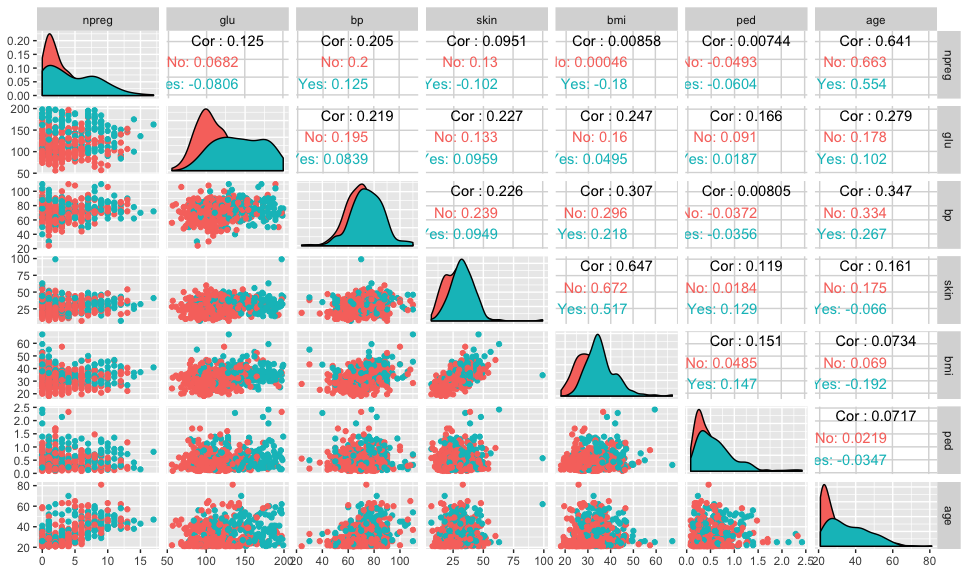
\includegraphics[scale=0.50]{plotgg}
\end{figure}
\newpage
\bibliographystyle{elsart-harv}
\bibliography{final_b}
 
\end{document}


